\documentclass[11pt,letterpaper]{article}
\usepackage{graphics}
\usepackage{fullpage}
\addtolength{\voffset}{0.5in}

%
%  Cool LaTeX resource:
%   http://en.wikibooks.org/wiki/LaTeX

\begin{document}
\title{Models of student learning and multimodel inference}
\author{Brett van de Sande}

\begin{abstract}
We compare several models of student learning of specific
skills with the goal of determing when a student has 
learned that skill.  We use Likelihood Theory to determine
which of several models best describes the acquisition
of skills associated with introductory physics.  Then we
use a multimodel approach to determine the relative probability
that a student has learned a given skill at a particular 
problem-solving step.  Finally, we relate this
approach with Hidden Markov model based approaches like
Bayesian Knowledge tracing.
\end{abstract}

\section{Introduction}

\section{A model of learning}

For each student and KC, the student has attempted some number of 
{\em steps} that involve that KC.   We will label
steps with $j$.  Usually a given step is associated
with a single user interface object (an equation, vector, etc.)  but
not always, since a student may attempt a particular problem solving
step, delete the object, and later attempt that solution step again.
Each step $j$ corresponds some some number of student-tutor 
{\em transactions}: attempts at constructing the associated object, 
or associated interactions with the Andes help system.  

%Next, we need a model of student learning for a particular KC.
%Since the policies chosen by the random-help version of Andes
%are different for each student,
%we need to determine the point of learning for each student.
For each KC and student, mark each step as ``correct'' if
the student completes the step correctly without any associated errors or 
requests for help; otherwise, the step is marked as ``incorrect.''
%
% From Kurt:
Thus, if each incorrect/correct step is marked with a 0/1, then
a single student's performance on a single KC is a bit string,
{\em exempli gratia} 00101011.


\section{Baysian Knowledge tracing}

The Bayesian Knowledge tracing model~\cite{anderson} has four parameters:
%
\begin{itemize}
   \item $P_0$ is the initial probability of knowing a skill.
   \item $P(G)$ is probability of guessing correctly, if the student        
         doesn't know the skill.
   \item $P(S)$ is probability of slips, if student does know the skill.
   \item $P(L)$ is probability of learning the skill if the student 
         does not know the skill.  Note that this is assumed to 
         be constant over steps.
\end{itemize}
%
Let $P_j$ be the probability that the student knows the skill at 
step $j$. According to the model,  $P_j$ can
be determined in terms of the previous opportunity:
%
\begin{equation}
          P_j = P_{j-1} + P(L)\left(1-P_{j-1}\right)
\end{equation}
%
According to this model, the probability that the student actually gets
opportunity $j$ correct is:
%
\begin{equation}
         P_j(C) = P(G)\left(1-P_j\right) + \left(1-P(S)\right) P_j \label{pnc}
\end{equation}
%
(Unlike the four model parameters above, there isn't a consistent
notation for $P_j(C)$ in the literature.)
This model can be exactly solved with solution: 
%
\begin{equation}
            P_j = 1-\left(1-P(L)\right)^j\left(1-P_0\right)
	    \label{sol}
\end{equation}
%
%
Substituting (\ref{sol}) into (\ref{pnc}), we get:
%
\begin{equation}
         P_j(C) = 1-P(S) -\left(1-P(S)-P(G)\right) \left(1-P_0\right)
                   \left(1-P(L)\right)^j \label{pncsoln}
\end{equation}
%
Note that the functional form of $P_j(C)$ is a function of {\em three}
parameters:  $P(S)$, $P(L)$, and $\left(1-P(S)-P(G)\right) \left(1-P_0\right)$.
This degeneracy of the model was first noticed by Beck and 
Chang~\cite{beckchang}.  In their paper, they notice that multiple
combinations of $P(G)$ and $P_0$ give exactly the same $P_j(C)$, but
fail to explain why this is the case.

The functional form of (\ref{pncsoln}) is an exponential.
If we define 
$A=\left(1-P(S)-P(G)\right) \left(1-P_0\right)$ and
$\beta=-\log(1-P(L))$, then we can rewrite (\ref{pncsoln}) in 
a clearer form:
%
\begin{equation}
         P_j(C) = 1-P(S) -A e^{-\beta j}
\end{equation}
%
So the graph of  $P_j(C)$ looks like the following:
%
\[
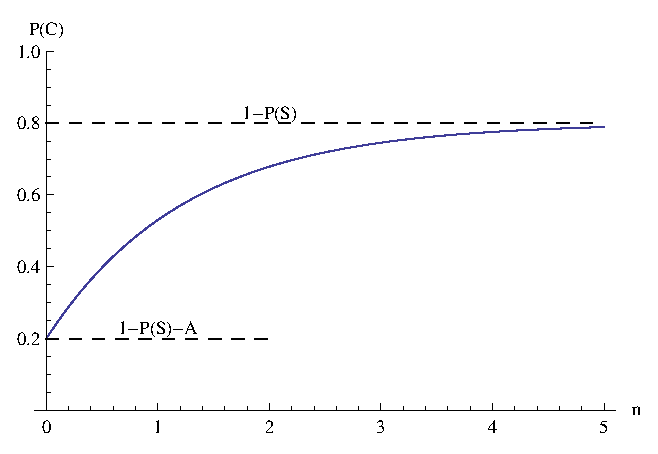
\includegraphics{exponential.eps}
\]
In conclusion, Baysian Knowledge tracing is equivalent to using
an exponential function with three parameters to fit the student data.

%Equations (1) and (2) of \cite{brunskill} 
%are equivalent to the first three equations in \cite{baker}
%\begin{eqnarray}
%   P(L_n|\mbox{correct}) &=& P(T)+\frac{\left(1-P(T)\right) P(L_{n-1})
%          \left(1-P(S)\right)}
%               {P(L_{n-1})\left(1-P(S)\right)+\left(1- P(L_{n-1})\right) P(G)}\\
%   P(L_n|\mbox{incorrect}) &=& P(T)+\frac{\left(1-P(T)\right) P(L_{n-1})
%          \P(S)\right}
%               {P(L_{n-1})P(S)+\left(1- P(L_{n-1})\right) \left(1-P(G)\right)}\\
%with the substitution:
%
%\begin{equation}
%         P(L_{n-1}) \to P(T)+\left(1-P(t)\right) p(L_t)
%\end{equation}
%
%This equivalence is from changing the order of updating
%student mastery and updating the estimate based on student
%response, as noted by the authors.  However, this raises
%a question for Equations (3) and (4) of \cite{brunskill}.
%Should the probability be taken before or after updating the
%student mastery:



\begin{thebibliography}{9}

\bibitem{anderson} 
  Corbett, A.\ T., Anderson, J.\ R. Knowledge Tracing:  Modeling 
the Acquisition of Procedural Knowledge.  \emph{User Modeling and
 User-Adapted Interaction}, 1995, 4, 253--278.

\bibitem{beckchang}
  Beck, J.\ E., Chang, K.-m.\ Identifiability: A Fundamental Problem of
  Student Modeling.
  \emph{Proceedings of the $11^{th}$ International Conference on User 
    Modeling}, 2007.

\bibitem{baker} Baker, R, Corbett, A., Aleven, V.,  Improving Contextual 
    Models of Guessing and Slipping with a Truncated Training Set. 
    First International Conference on Educational Data Mining. 2008. 

\bibitem{brunskill}
   Lee, J.\ I., Brunskill, E.\ The impact of Individualizing Student 
  Modesls on Necessary Practice Opportunities.  EDM, 2012.

\end{thebibliography}




\end{document}